\documentclass[11pt]{report}

% sensible specification of margins, etc.
\usepackage[paperwidth=8.5in,paperheight=11in]{geometry}
\geometry{inner=1.0in, outer=1.5in, top=1.0in, bottom=0.5in,
  includefoot}
\geometry{twoside}

% for displaying graphics
\usepackage[]{graphicx}
% where can I find the graphics that will be imported for this version
\graphicspath{{./figures/}}

% for wrapping figures
\usepackage{wrapfig}

% running headers
\usepackage{fancyhdr}
\fancyhead{}
\fancyfoot{}
\fancyhead[CO,CE]{---Draft---}
\fancyhead[LO,RE]{\it Ginga FITS Viewer and Toolkit Manual}
\fancyhead[LE,RO]{\slshape \rightmark}
\fancyfoot[C]{\thepage}
%\fancyfoot[LE,RO] {\slshape \rightmark}
%\fancyfoot[LO,RE] {\slshape \leftmark}

% for Japanese language support, comment out if this causes a problem
\usepackage{xeCJK}
\setCJKmainfont{TakaoMincho}

% use modern and attractive fonts
\usepackage{fontspec}
\setmainfont[Mapping=tex-text]{Times New Roman}
\setsansfont[Mapping=tex-text]{Arial}
%\setmonofont[Scale=0.85]{Courier New}
\setmonofont[]{Courier New}
%% \setmainfont[Mapping=tex-text]{Bitstream Vera Serif}
%% \setsansfont[Mapping=tex-text]{Bitstream Vera Sans}
%% \setmonofont[Scale=0.85]{Bitstream Vera Sans Mono}

% Save space in headings
%% \usepackage[small,compact]{titlesec}
%% \titlespacing{\section}{0pt}{*0}{*0}
%% \titlespacing{\subsection}{0pt}{*0}{*0}
%% \titlespacing{\subsubsection}{0pt}{*0}{*0}

% provides itemize* environment
\usepackage{mdwlist}
% for tables with paragraphs
\usepackage{tabularx}

% for code listings
\usepackage{listings}
\usepackage{color}
\usepackage{textcomp}
\lstset{
	%backgroundcolor=\color{lbcolor},
	tabsize=4,
	%rulecolor=,
	language=Python,
        basicstyle=\scriptsize,
        upquote=true,
        aboveskip={1.5\baselineskip},
        columns=fixed,
        extendedchars=true,
        breaklines=true,
        prebreak = \raisebox{0ex}[0ex][0ex]{\ensuremath{\hookleftarrow}},
        %frame=single,
        showtabs=false,
        showspaces=false,
        showstringspaces=false,
        identifierstyle=\ttfamily,
        keywordstyle=\color[rgb]{0,0,1},
        commentstyle=\color[rgb]{0.9,0.0,0.133},
        stringstyle=\color[rgb]{0.127,0.5126,0.941},
}
\usepackage{verbatim}
\newenvironment{myverbatim}
  {\setlength{\parskip}{0pt}\verbatim}
  {\endverbatim}

%\raggedright

\setlength{\parindent}{0cm}
\setlength{\parskip}{1em plus0.5em minus0.5em}

\setlength{\marginparsep}{0.35in}
\setlength{\marginparwidth}{1.5in}

\title{The Ginga Viewer and Toolkit Manual} 
\author{Eric Jeschke\\
{\tt eric@naoj.org},\\
 (alt) {\tt eric@redskiesatnight.com}\\
\\
Observation Control Software Group\\
Subaru Telescope\\
National Astronomical Observatory of Japan}

\pagestyle{fancy}    


\begin{document} 

\maketitle 

\begin{abstract}
Ginga is a toolkit for building viewers for scientific data in Python,
particularly astromonical data.  It includes a reference viewer for
viewing FITS (Flexible Image Transport System) files.
The Ginga viewer is based on a new display object which supports 
zooming and panning, color and intensity mapping, a choice of several
automatic cut levels algorithms and canvases for plotting scalable
geometric forms.  In addition to this widget, the fits viewer provides a
flexible plugin framework for extending the viewer with many different
features.  A fairly complete set of standard plugins are provided
for features that we expect from a modern viewer: panning and zooming
windows, star catalog access, cuts, star pick/fwhm, thumbnails, etc.
\end{abstract}

\tableofcontents
\setcounter{tocdepth}{3}

\newpage

%%%%%%%%%%%%%%%%%%%%%%%%%%%%%%%%%%%%%%%%%%%%%%%%%%%%%%%%%%%%% 
\chapter{Introduction}
\label{sh:intro}
\begin{center}
\Huge{銀河}
\end{center}

%%%%%%%%%%%%%%%%%%%%%%%%%%%%%%%%%%%%%%%%%%%%%%%%%%%%%%%%%%%%% 

\section{About}
\label{sec:about}
\emph{Ginga} is a toolkit designed for building viewers for 
scientific image data in Python, visualizing 2D pixel data in
{\tt numpy} arrays.  It was originally designed to to view astronomical
data such as loaded from files based on the FITS (Flexible Image
Transport System) file format.  It is written and is maintained by
software engineers at the Subaru Telescope, National Astronomical
Observatory of Japan.

\subsection{Features}
The Ginga toolkit centers around an image display object which supports 
zooming and panning, color and intensity mapping, a choice of several
automatic cut levels algorithms and canvases for plotting scalable
geometric forms.  In addition to this widget, a general purpose
``reference'' FITS viewer is provided, based on a plugin framework.
A fairly complete set of ``standard'' plugins are provided for features
that we expect from a modern FITS viewer: panning and zooming windows,
star catalog access, cuts, star pick/fwhm, thumbnails, etc. 

\section{Core Concepts}
Ginga operation and documentation is organized around a few core
concepts and associated nomenclature.  Knowing these may aid in
understanding the rest of the documentation. 

\subsection{Workspaces}
Ginga has a flexible panel/workspace layout algorithm that allows a
lot of customization into the appearance of the program.  The majority
of the interface is constructed as hierchical series of horizontally or
vertically-adjustable panels.  At the terminus of each panel is a
\emph{workspace}.
Each workspace is typically
implemented by a GUI toolkit container widget such as a notebook widget,
where each item in the workspace is identified by a tab.  Workspaces can
be nested, so a tab might contain yet another nested set of tabs, and so
on\footnote{Note that workspaces may be implemented by several types of 
  container widgets such as fixed position subwindows, sliding panes,
  MDI-style subwindows, etc.  A notebook widget is simply the most
  common (default) case.}. 
Tabs can be freely dragged between workspaces, or out onto the desktop,
forming a new, detached workspace.

In its default configuration, Ginga starts up with a
single row (horizontal) panel of three workspaces, as shown in
Figure \ref{fig:gingadefault}.
This panel is sandwiched vertically between a menu bar and a status bar.

% fig: showing the default configuration
\begin{figure}
  \begin{center}
    \begin{tabular}{c}
      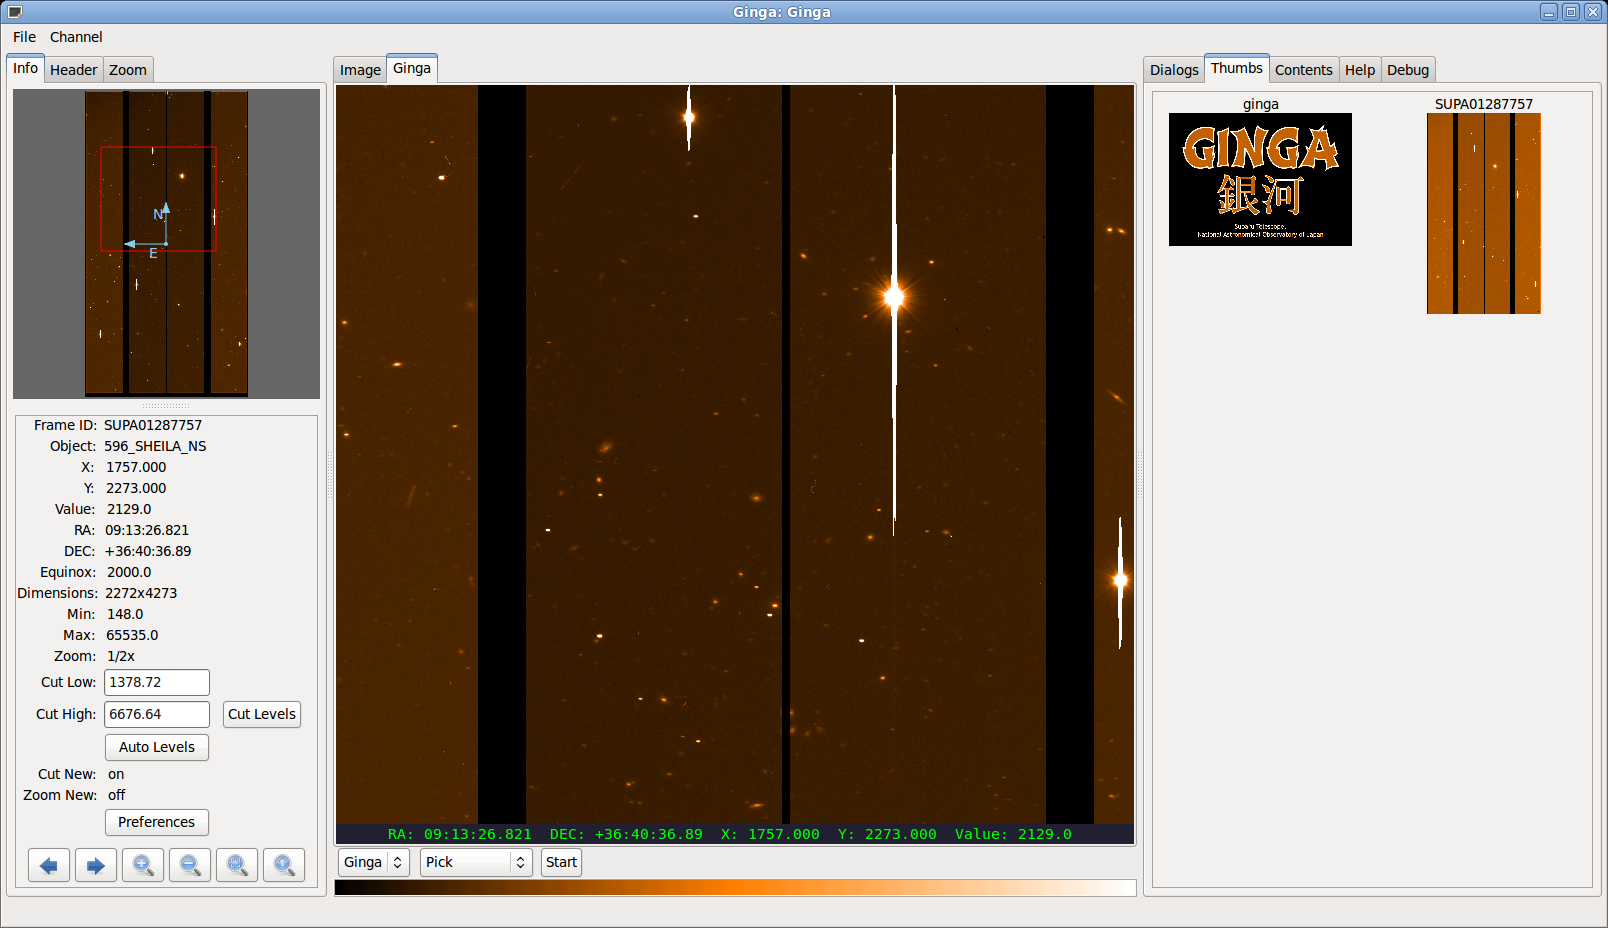
\includegraphics[width=6in]{gingadefault.png}
    \end{tabular}
  \end{center}
  \caption[example] 
%% %>>>> use \label inside caption to get Fig. number with \ref{}
          { \label{fig:gingadefault} 
            A typical Ginga layout.} 
\end{figure} 

The layout of the workspaces is controlled by a table in the Ginga
startup script.  By changing this table the layout can be substantially
altered. 

\subsection{Channels}
Another core tenet of Ginga is that image content is organized
into {\em channels}.  A channel can be thought of as simply a named
category under which similar types of images might be organized.
Examples: 
\begin{itemize*}
\item a channel for each type of instrument at a telescope;
\item a channel for each observation or calibration target;
\item channels based on time or program or proposal identifier;
\item etc.
\end{itemize*}
If no channels are specified when Ginga starts up it simply creates a
default channel named ``Image''.  New channels can be created using the
{\tt Channel/Add channel} menu item.

In the case where multiple channels are present, they are usually visually
organized as tabs within the central workspace of the interface.  To
change channels you simply click on the tab of the channel you want to
view.  There is also a channel selector in the plugin manager toolbar at
the bottom of the center pane.  Using the drop-down menu or by simply
scrolling the mouse wheel on the control you can change the channel.

Channels occupy a flat namespace; i.e. there is no sense of a hierarchy
of channels.
By default, images are loaded into the same channel you are currently
viewing (unless your viewer has been customized to load images according
to special rules).
To keep images organized, simply change to the desired channel before
opening a new image. 

Many preferences in Ginga are set on a per-channel basis.  A new channel
will generally ``inherit'' the settings for the generic ``Image''
channel until new preferences are defined and saved.

\subsection{Plugins}
Most functionality in Ginga is achieved through the use of a plugin
architecture.
In this manual we will also use the word {\em operation} to describe activating
a plugin.  For example, a pick operation would invoke and use the Pick
plugin.  The plugins are each described in more detail in Chapter 
\ref{ch:plugins}.  Plugins are written as encapsulated Python modules
that are loaded dynamically when Ginga starts.  There is an API for
programming plugins (see Chapter \ref{ch:plugins}).  

A plugin may or may not have an associated Graphical User Interface (GUI).
For those that do have a visible interface, the Ginga startup script
can map them to certain workspaces.  By manipulating this mapping (along
with the workspace layout) extremely customized and flexible layouts can
be achieved.  
In Figure \ref{fig:gingadefault} the left workspace contains three
global plugin UIs: the Info, Header and Zoom panes.  The middle workspace
holds all the viewing panes for each channel.  The right workspace has
the Dialogs, Thumbs, Contents and Help panes.  The operation of these
plugins is described in Chapter \ref{ch:plugins}. 

\section{General operation}
\label{sec:generalop}

\subsection{Terminology}
In this manual we will use the following terms to describe operations
with the mouse:
\begin{itemize*}
\item \emph{Click} or \emph{Left-click} means to click on an item with
  the left mouse button;
\item \emph{Drag} or \emph{Left-drag} means to click, hold and drag with
  the left mouse button;
\item \emph{Scroll} means to scroll with the middle mouse wheel;
\item \emph{Scroll-click} means to click with the middle mouse wheel/button;
\item \emph{Scroll-drag} means to click, hold and drag with the middle
  mouse wheel/button; 
\item \emph{Right-click} means to click on an item with the right mouse
  button; 
\item \emph{Right-drag} means to click, hold and drag with the right
  mouse button.
\end{itemize*}

Mouse operations are also modified by the keyboard buttons {\tt Shift}
and {\tt Ctrl}.  \emph{Shift-click} means to press \emph{and hold} the
{\tt Shift} key while clicking with left mouse button,
\emph{Shift-right-click} is the same using the right mouse button,
etc.
Some mouse-controlled operations in Ginga are initiated by a key stroke.
In these cases the key is pressed and released (not held), and then the
mouse is used to control the operation.  Such operations are either
terminated by releasing the mouse button (if the operation employs a
drag), clicking on the image or pressing the {\tt Esc} key (if not a
drag operation).

\subsection{Loading a FITS image file}
There are several ways to load a file into Ginga.
\begin{itemize}
\item Ginga supports drag-and-drop in a typical desktop environment, so
  you can simply drag and drop files from a graphical file manager such
  as the Mac finder or Linux nautilus onto the main FITS viewing pane to
 load the image.
\item Another way is to invoke the FBrowser plugin, which opens in the Dialogs
 tab.  The plugin pane shows file and folder contents and allows
 navigation up and down the filesystem hierarchy by double-clicking on
 folder names.   Simply navigate to the location of the FITS file and
 double-click on the file name to load it.
\item Use the {\tt Load Image} entry from the {\tt File} menu on
  the main menu bar at the top of the window.  This opens a standard file
  dialog popup window where you can navigate to the file you wish to load.
\end{itemize}

\subsection{Zooming and panning}
The display object used throughout most of the Ginga panels has built-in
support for zooming and panning.  Appendix \ref{app:mousekbdref} has the
complete listing of default keyboard and mouse bindings.  
Briefly, the scroll wheel of the mouse can be used to zoom in and out,
along with the {\tt +} and {\tt -} keys.  The backquote key will fit the
image to the window.  Digit keys ({\tt 1, 2}, etc) will zoom in to the
corresponding zoom level, while holding Shift and pressing a zoom key
zooms out to the corresponding level.

When zoomed in, panning is enabled.  Panning takes two forms.
\emph{Free panning} allows scrolling around the entire image by mapping
the entire image boundaries to the window boundaries.  For example,
moving the mouse to the upper right-hand corner of the window will pan to
the upper right hand corner of the image, etc.  There are two ways to
initiate a free pan: Scroll-dragging (pressing the mouse scroll wheel
and dragging) or press and release {\tt q} and then Left-drag.
\emph{Proportional panning} or ``drag panning'' pans the image in direct
proportion to the distance the mouse is moved; a common idiom is
dragging the image canvas in the direction you want to move it under the
window.  To utilize a proportional pan, Ctrl-drag the canvas.  The Pan
plugin (usually embedded under the {\tt Info} tab) shows the outline of
the current pan position as a rectangle on a small version of the whole
image.  Dragging this outline will also pan the image in the main window.

Panning in Ginga is based on an (X, Y) coordinate known as the 
\emph{pan position}.  The pan position determines what Ginga will 
try to keep in the middle of the window as the image is zoomed.  
When zoomed out, one can Shift-click on a particular point in the image
(or press the {\tt p} key while hovering over a spot),
setting the pan position.  Zooming afterward will keep the pan
position in the center of the window.

Ginga has an auto zoom feature to automatically fit newly loaded images
to the window, similar to what happens when the backquote key is
pressed.  See section \ref{pref:zoomnew} for details.

\subsection{Setting cut levels}
When visualizing pixel data with an arbitrary pixel value range, the
range is mapped into a bytescaled range spanning from black to white
based on the low and high \emph{cut levels} defined in the view object.
These cut levels can be set manually by the user or automatically based
on a selection of algorithms supported by the view.

\subsubsection{Manually setting cut levels}
There are several ways to manually set the cut levels:
\begin{itemize}
\item The ``Cut Low'' and ``Cut High'' boxes in the Info plugin panel
  can be used.  The current values are shown to the left; simply type a
  new value in the corresponding box and press Enter or click the ``Cut
  Levels'' button below.
\item Pressing and releasing the less than ({\tt \textless}) or greater than
 ({\tt \textgreater}) key
  will invoke an interactive cut levels, for the low and high value
  respectively.  After releasing the key, click and drag the mouse
  horizontally in the window to interactively set the level--when you
  reach the desired level, release the mouse button.
\item Pressing and releasing the period ({\tt \.}) key will invoke a 
  dual (high and low) interactive cut levels.  After releasing the key,
  click and drag the mouse horizontally in the window to interactively
  set the high level, and vertically to set the low level--when you
  reach the desired levels, release the mouse button.
\end{itemize}

\subsubsection{Automatically setting cut levels}
Ginga can algorithmically estimate and set the cut levels--a so called
``auto (cut) levels''.  To activate the auto levels:
\begin{itemize}
\item Click the ``Auto Levels'' button in the Info plugin panel, or
\item Press the ({\tt a}) key when the viewing widget has the focus.
\end{itemize}

The auto cut levels feature is controlled by several factors in the
preferences, including the choice of algorithm and some parameters to
the algorithm.  See section \ref{sec:autocuts} for details.
Ginga can also automatically set the cut levels for new images displayed
in the view.  See section \ref{pref:cutnew} for details.

\subsection{Manipulating the color map}


%%%%%%%%%%%%%%%%%%%%%%%%%%%%%%%%%%%%%%%%%%%%%%%%%%%%%%%%%%%%% 
\chapter{Plugins}
\label{ch:plugins}
%%%%%%%%%%%%%%%%%%%%%%%%%%%%%%%%%%%%%%%%%%%%%%%%%%%%%%%%%%%%% 
Ginga is written so that most of the functionality of the program is
achieved through the use of plugins.  This modular approach allows a
large degree of flexiblity and customization, as well as making overall
design and maintenance of the program simpler.

Plugins are divided into two types: global and local.  A global plugin
has a single instance shared by all channels, while a local plugin
creates a unique instance for each channel.  If you switch channels, a
global plugin will respond to the change by updating itself,
while a local plugin will remain unchanged if the channel is switched,
because its operation is specific to a given channel.

This chapter describes the set of plugins that come with Ginga.  Those
interested in writing their own custom plugins should refer to chapter
\ref{ch:writingplugins}. 

\section{Global plugins}

\newpage
\subsection{Pan}
\begin{wrapfigure}{o}{2.5in}
  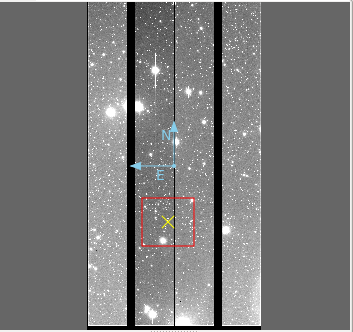
\includegraphics[width=2.5in]{pan-plugin.png}
  \caption[example] 
          { \label{fig:pan-plugin} 
            The Pan plugin.} 
\end{wrapfigure} 
The Pan plugin provides a small panning image that gives an overall
``birds-eye'' view of the channel image that last had the focus.  If the
channel image is zoomed in 2X or greater then the pan region is shown
graphically in the Pan image by a rectangle.  The channel image can be
panned by clicking and/or dragging to place the rectangle.  You can also
use the scroll wheel in the Pan image to zoom the channel image.

The color/intensity map and cut levels of the Pan image are updated
when they are changed in the corresponding channel image.
The Pan image also displays the World Coordinate System compass, if
valid WCS metadata is present in the FITS HDU being viewed in the
channel.

\newpage
\subsection{Info}
\begin{wrapfigure}{o}{2.5in}
  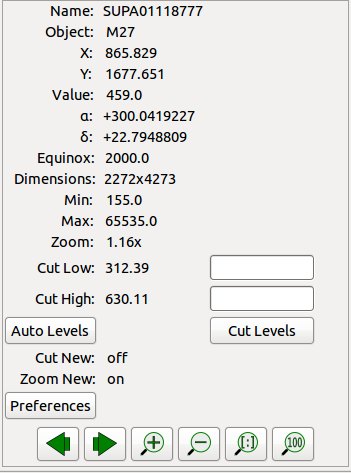
\includegraphics[width=2.5in]{info-plugin.png}
  \caption[example] 
          { \label{fig:info-plugin} 
            The Info plugin.} 
\end{wrapfigure} 
The Info plugin provides a pane of commonly useful metadata about the
associated channel image.  Common information includes some
FITS header values, the equinox, dimensions of the image, minimum and
maximum values and the zoom level.  As the cursor is moved around the
image, the X, Y, Value, RA and DEC values are updated to reflect the
value under the cursor.

At the bottom of the Info interface are the cut levels controls. Here
the low and high cut levels are shown and can be adjusted.  Finally,
there is a Preferences button that will take the user quickly to the
Preferences plugin for the channel.

The Pan and Info plugins are typically combined under the Info tab in
the user interface.  Below the Info plugin appear several buttons that
can be used to zoom the image or to navigate between images in the
history of the current channel.

\newpage
\subsection{Header}
\begin{wrapfigure}{o}{2.5in}
  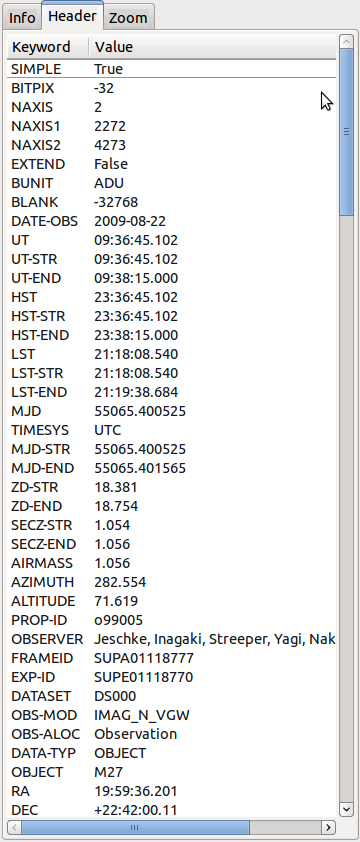
\includegraphics[width=2.5in]{header-plugin.png}
  \caption[example] 
          { \label{fig:header-plugin} 
            The Header plugin.} 
\end{wrapfigure} 
The Header plugin shows the FITS keyword metadata from the image.
Initially only the primary HDU metadata is shown.  However, in
conjunction with the MultiDim plugin the metadata for other HDUs will be
shown.  See the MultiDim plugin description for details.

Clicking on a column header will sort the table by values in that
column, which may be useful for quickly locating a particular keyword.

\newpage
\subsection{Zoom}
\begin{wrapfigure}{o}{2.5in}
  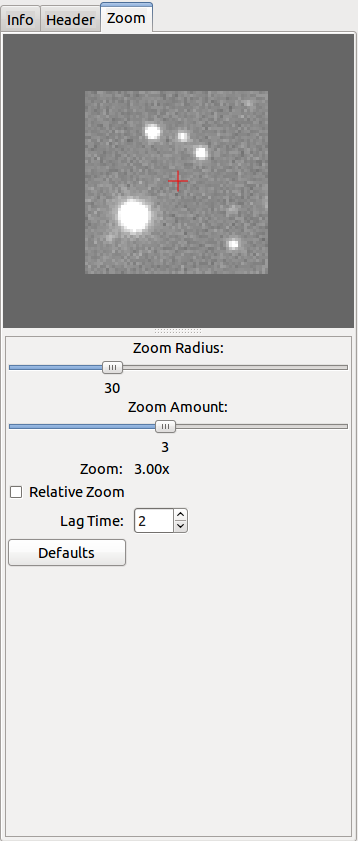
\includegraphics[width=2.5in]{zoom-plugin.png}
  \caption[example] 
          { \label{fig:zoom-plugin} 
            The Zoom plugin.} 
\end{wrapfigure} 
The Zoom plugin shows an enlarged image of a cutout region centered
under the cursor position in the associated channel image.  As the
cursor is moved around the image the zoom image updates to allow close
inspection of the pixels or precise control in conjunction with other
plugin operations.

The size of the cutout radius can be adjusted by the slider below the
zoom image labeled ``Zoom Radius''. The default radius is 30 pixels,
making a 61x61 zoom image.  The magnification can be changed by
adjusting the ``Zoom Amount'' slider.
Above zero, the zoom range corresponds to logical increments: 1=1X,
2=2X, etc.  The zoom scale is discontinuous at the 0 and -1 settings,
which are equivalent to 1X.  Settings below -1 correspond to zooming out,
e.g. -2=1/2, -3=1/3, etc. 

Two modes of operation are possible: absolute and relative zoom.  In
absolute mode, the zoom amount controls exactly the zoom level shown in
the cutout: for example, the channel image may be zoomed into 10X, but
the zoom image will only show a 3X image if the zoom amount is set to
3X.
In relative mode, the zoom amount setting is interpreted as relative to
the zoom setting of the channel image.  If the zoom amount is set to 3X
and the channel image is zoomed to 10X then the zoom image shown will be
10+3=13X.  Note that the zoom amount setting can be negative, so a
setting of -3X with a 10X zoom in the channel image will produce a
10-3=7X zoom image.
In both modes the minimum and maximum zoom level of the zoom image is
limited by the Min Zoom and Max Zoom settings, which are
user-adjustable.  

\newpage
\subsection{Thumbs}
\begin{wrapfigure}{o}{2.5in}
  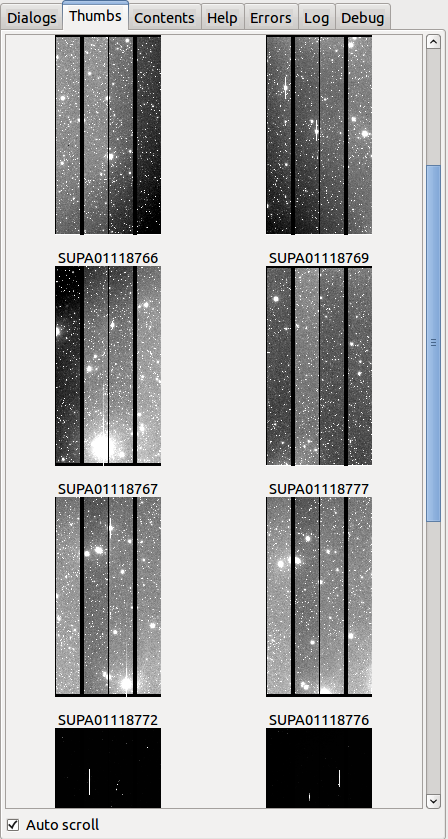
\includegraphics[width=2.5in]{thumbs-plugin.png}
  \caption[example] 
          { \label{fig:thumbs-plugin} 
            The Thumbs plugin.} 
\end{wrapfigure} 
The Thumbs plugin provides an index of all images viewed since the
program was started.  Clicking on a thumbnail navigates you directly to
that image.  Thumbs appear in cronological viewing history, with the
newest images at the bottom and the oldest at the top.  Hovering the
cursor over a thumbnail will show a tooltip that contains a couple of
useful pieces of metadata from the image.

\newpage
\subsection{Contents}
The Contents plugin provides a table of contents like interface for all
the images viewed since the program was started.  Unlike Thumbs,
Contents is sorted by channel, and then by image name.  The contents
also shows some common metadata from the image.

\section{Local plugins}

An {\em operation} is the activation of a local plugin to perform some
function.  Operations can the started and controlled in two ways:
graphically, or using the keyboard shortcuts.  The plugin manager
toolbar at the bottom of the center pane is the graphical way to start
an operation.  


\subsection{Pick}
\subsection{Ruler}
\subsection{MultiDim}
\subsection{Cuts}
\subsection{Histogram}
\subsection{PixTable}
\subsection{Preferences}
The Preferences plugin sets the preferences on a per-channel basis.
The preferences for a given channel are inherited from the ``Image''
channel until they are explicitly set and saved using this plugin.

\newpage
\subsubsection{Color Preferences}
\begin{figure}
  \begin{center}
    \begin{tabular}{c}
      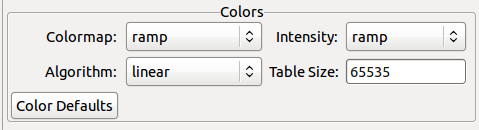
\includegraphics[width=4in]{cmap-prefs.png}
    \end{tabular}
  \end{center}
  \caption[example] 
          { \label{fig:prefs-colors} 
            The color map preferences.} 
\end{figure} 
The Colors preferences, shown in Fig. \ref{fig:prefs-colors}, controls
the preferences used for the color map, intensity map, color mapping
algorithm and color hash table size.
Together these control the mapping of data values into a 24-bpp RGB
visual representation.

The ``Colormap'' control selects which color map should be loaded and
used.  Click the control to show the list, or simply scroll the mouse
wheel while hovering the cursor over the control.

The ``Intensity'' control selects which intensity map should be used
with the color map.  The intensity map is applied just before the color
map, and can be used to change the standard linear scale of values into
an inverted scale, logarithmic, etc.

The ``Algorithm'' control is used to set the initial mapping of pixel
values into a hash table.

The ``Table Size'' control sets the size of the hash table used to map
pixel values.

Ginga comes with a good selection of color maps, but should you want
more you can add custom ones or, if {\tt matplotlib} is installed, you
can load all the ones that it has installed.  See Chapter
\ref{ch:customizing} for details.

\subsubsection{Zoom Preferences}
\begin{figure}
  \begin{center}
    \begin{tabular}{c}
      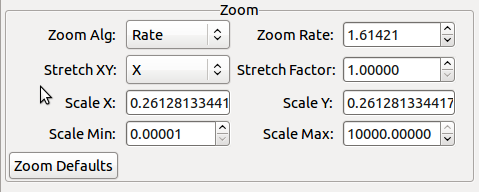
\includegraphics[width=4in]{zoom-prefs.png}
    \end{tabular}
  \end{center}
  \caption[example] 
          { \label{fig:prefs-zoom} 
            The zoom preferences.} 
\end{figure} 
The Zoom preferences, shown in Fig. \ref{fig:prefs-zoom}, controls
Ginga's zooming/scaling behavior.

Ginga supports two zoom algorithms, chosen using the ``Zoom Alg'' control:
\begin{itemize}
\item The \emph{step} algorithm zooms the image inwards in discrete
  steps of 1X, 2X, 3X, etc. or outwards in steps of 1/2X, 1/3X, 1/4X,
  etc.  This algorithm results in the least artifacts visually, but is a
  bit slower to zoom over wide ranges when using a scrolling motion
  because more ''throw'' is required to achieve a large zoom change
  (this is not the case if one uses of the shortcut zoom keys, such as
  the digit keys). 
\item The \emph{rate} algorithm zooms the image by advancing the scaling at
  a rate defined by the value in the Zoom Rate box.  This rate defaults
  to the square root of 2.  Larger numbers cause larger changes in scale
  between zoom levels.  If you like to zoom your images rapidly, at a
  small cost in image quality, you would likely want to choose this
  option. 
\end{itemize}
Note that regardless of which method is chosen for the zoom algorithm,
the zoom can be controlled by holding down Ctrl (coarse) or Shift
(fine) while scrolling to constrain the zoom rate.

The ``Stretch XY'' control can be used to stretch one of the axes (X or
Y) relative to the other.  Select an axis with this control and roll the
scroll wheel while hovering over the ``Stretch Factor'' control to
stretch the pixels in the selected axis.

The ``Scale X'' and ``Scale Y'' controls offer direct access to the
underlying scaling, bypassing the discrete zoom steps.  Here exact
values can be typed to scale the image.  Conversely, you will see these
values change as the image is zoomed.

The ``Scale Min'' and ``Scale Max'' controls can be used to place a
limit on how much the image can be scaled.

The ``Zoom Defaults'' button will restore the controls to the Ginga
default values. 

\subsubsection{Pan Preferences}
\begin{figure}
  \begin{center}
    \begin{tabular}{c}
      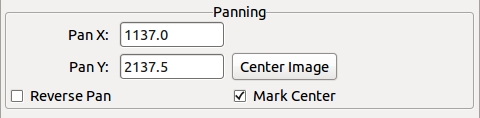
\includegraphics[width=4in]{pan-prefs.png}
    \end{tabular}
  \end{center}
  \caption[example] 
          { \label{fig:prefs-pan} 
            The pan preferences.} 
\end{figure} 
The Pan preferences, shown in Fig. \ref{fig:prefs-pan}, controls
Ginga's panning behavior.

The ``Pan X'' and ``Pan Y'' controls offer direct access to set the pan
position in the image (the part of the image located at the center of
the window)--you can see them change as you pan around the image.

The ``Center Image'' button sets the pan position to the center of the
image, as calculated by halving the dimensions in X and Y.

Checking the ``Reverse Pan'' box reverses the sense of zooming and
panning in Ginga: the scroll wheel will zoom the image in the opposite
direction of normal, and when free panning you move to the opposite
corner of the window to pan to the corner that you want to see.  
This control is largely for the benefit of those used to the scrolling
and zooming behavior of some older FITS viewers.

The ``Mark Center'' check box, when checked, will cause Ginga to draw a
small reticle in the center of the image.  This is useful for knowing
the pan position and for debugging.

\subsubsection{Transform Preferences}
\begin{figure}
  \begin{center}
    \begin{tabular}{c}
      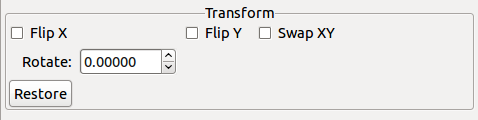
\includegraphics[width=4in]{transform-prefs.png}
    \end{tabular}
  \end{center}
  \caption[example] 
          { \label{fig:prefs-transform} 
            The transform preferences.} 
\end{figure} 
The Transform preferences, shown in Fig. \ref{fig:prefs-transform},
allows one to transform the view of the image by flipping the view in X
or Y, swapping the X and Y axes, or rotating the image in arbitrary amounts.

The ``Flip X'' and ``Flip Y'' checkboxes cause the image view to be
flipped in the corresponding axis.

The ``Swap XY'' checkbox causes the image view to be altered by swapping
the X and Y axes.  This can be combined with Flip X and Flip Y to rotate
the image in 90 degree increments.  These views will render more quickly
than arbitrary rotations using the Rotate control. 

The ``Rotate'' control will rotate the image view an arbitrary amount.
The value should be specified in degrees.  Rotate can be specified in
conjunction with flipping and swapping.

The ``Restore'' button will restore the view to the default view, which
is unflipped, unswapped and unrotated.

\subsubsection{Auto Cuts Preferences}
\label{sec:autocuts}
\begin{figure}
  \begin{center}
    \begin{tabular}{c}
      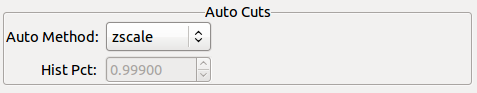
\includegraphics[width=4in]{autocuts-prefs.png}
    \end{tabular}
  \end{center}
  \caption[example] 
          { \label{fig:prefs-autocuts} 
            The auto cuts preferences.} 
\end{figure} 
The Auto Cuts preferences, shown in Fig. \ref{fig:prefs-autocuts},
controls the calculation of auto cut levels for the view when the auto
cut levels button or key is pressed, or when loading a new image with
auto cuts enabled. 

The ``Auto Method'' control is used to choose which auto cuts algorithm
used: `minmax' (minimum maximum values), `histogram' (based on an image
histogram), `stddev' (based on the standard deviation of pixel values), or 
`zscale' (based on the ZSCALE algorithm popularized by IRAF).  Note that,
currently, there is limited GUI support for additional parameters to the
algorithms, with the exception of the ``Hist Pct''--percentage of the
histogram used in the case of method `histogram'.

\subsubsection{WCS Preferences}
\begin{figure}
  \begin{center}
    \begin{tabular}{c}
      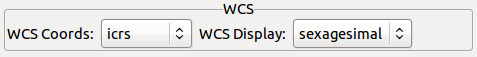
\includegraphics[width=4in]{wcs-prefs.png}
    \end{tabular}
  \end{center}
  \caption[example] 
          { \label{fig:prefs-wcs} 
            The world coordinate system preferences.} 
\end{figure} 
The WCS preferences, shown in Fig. \ref{fig:prefs-wcs}, controls the
display preferences for the World Coordinate System calculations used to
report the cursor position in the image.

The ``WCS Coords'' control is used to select the coordinate system in
which to display the result.

The ``WCS Display'' control is used to select a sexagesimal (H:M:S)
readout or a decimal degrees readout.

\subsubsection{New Image Preferences}
\begin{figure}
  \begin{center}
    \begin{tabular}{c}
      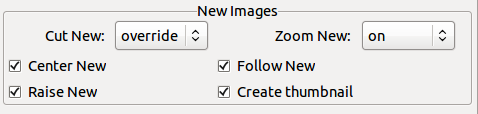
\includegraphics[width=4in]{newimages-prefs.png}
    \end{tabular}
  \end{center}
  \caption[example] 
          { \label{fig:prefs-newimages} 
            The new images preferences.} 
\end{figure} 
The New Images preferences, shown in Fig. \ref{fig:prefs-newimages},
controls how Ginga reacts when a new image is loaded into the channel.
This includes when an older image is revisited by clicking on its
thumbnail in the Thumbs plugin pane.

\label{pref:cutnew}
The ``Cut New'' setting controls whether an automatic cut levels
calculation should be performed on the new image, or whether the
currently set cut levels should be applied.  The possible settings are:
\begin{itemize}
\item `on': calculate a new cut levels always;
\item `override': calculate a new cut levels until the user overrides
  it by manually setting a cut levels, then turn `off'; or
\item `off': always use the currently set cut levels.
\end{itemize}
The `override' setting is provided for the convenience of having an
automatic cut levels, while preventing a manually set cuts from being
overrided when a new image is ingested.  The semicolon key is used to
toggle the mode back to override, while colon will set the preference to
`on'. 

\label{pref:zoomnew}
The ``Zoom New'' setting controls whether a newly visited image should
be zoomed to fit the window.  There are three possible values: `on',
`override', and `off':
\begin{itemize}
\item `on': the new image is always zoomed to fit;
\item `override': images are automatically fitted until the zoom level is
changed manually--then the mode automatically changes to `off', or
\item `off': always use the currently set zoom levels.
\end{itemize}
The `override' setting is provided for the convenience of having an
automatic zoom, while preventing a manually set zoom level from being
overrided when a new image is ingested.  The apostrophe (aka ``single
quote'') key is used to toggle the mode back to override, while quote
(aka ``double quote'') will set the preference to `on'. 

The ``Center New'' box, if checked, will cause newly visited images to
always have the pan position reset to the center of the image.  If
unchecked, the pan position is unchanged from the previous image.

The ``Follow New'' setting is used to control whether Ginga will change
the display if a new image is loaded into the channel.  If unchecked,
the image is loaded (as seen, for example, by its appearance in the
Thumbs tab), but the display will not change to the new image.  This
setting is useful in cases where new images are being loaded by some
automated means into a channel and the user wishes to study the current
image without being interrupted.

The ``Raise New'' setting controls whether Ginga will raise the tab of a
channel when an image is loaded into that channel.  If unchecked then
Ginga will not raise the tab when an image is loaded into that
particular channel.

The ``Create Thumbnail'' setting controls whether Ginga will create a
thumbnail for images loaded into that channel.  In cases where many
images are being loaded into a channel frequently (e.g. a low frequency
video feed) it may be undesirable to create thumbnails for all of them.

\subsection{Catalog}
\subsection{Drawing}
\subsection{FBrowser}
\subsection{WBrowser}

\section{Optional Plugins}
\label{sec:optionalplugins}
There are a number of plugins distributed with Ginga that are not loaded
by default.  In keeping with the ``small is beautiful'' mantra, these
plugins can be loaded when needed.

\subsection{Remote Control}
\label{sec:remotecontrol}
You may find that you have a need to control Ginga remotely.  For
example, you want to invoke the loading of images, or performing
operations on images, etc.  Like many other aspects, Ginga delegates this
task to a plugin: RC.  
Because remote control of Ginga is handled by a plugin, you can easily
change the types of operations that can be done, or completely change
the protocol used.

The remote control module is not loaded by default.  To load it, specify
the command line option:
\begin{verbatim}
--modules=RC
\end{verbatim}

You can then control Ginga from the {\tt grc} program located in the 
{\tt scripts} directory.  Some examples:
\begin{verbatim}
 Create a new channel:
 $ grc ginga add_channel FOO
 
 Load a file:
 $ grc ginga load FOO /home/eric/testdata/SPCAM/SUPA01118797.fits

 Cut levels:
 $ grc channel FOO cut_levels 163 1300

 Auto cut levels:
 $ grc channel FOO auto_levels

 Zoom to fit:
 $ grc channel FOO zoom_fit
 
 Transform:
 $ grc channel FOO transform 1 0 1
\end{verbatim}

Almost any method on the Ginga shell or a channel can be invoked from
the remote plugin.  Methods on the shell can be called like this:
\begin{verbatim}
 $ grc ginga <method> <arg1> <arg2> ...
\end{verbatim}

Channel methods can be called like this:

\begin{verbatim}
 $ grc channel <chname> <method> <arg1> <arg2> ...
\end{verbatim}

Built in help is available for showing method docstrings:
\begin{verbatim}
 Show example usage:
 $ grc help

 Show help for a specific ginga method:
 $ grc help ginga <method>

 Show help for a specific channel method:
 $ grc help channel <chname> <method>
\end{verbatim}

Calls can be made from a remote host by simply adding the options
\begin{verbatim}
   --host=<hostname> --port=9000
\end{verbatim}
to the command line.

In some cases, you may need to resort to shell escapes to be able to
pass certain characters to Ginga.  For example, a leading dash character is
usually interpreted as a program option.  In order to pass a signed
integer you may need to do something like:
\begin{verbatim}
 Zoom to a specific level:
 $ grc -- channel FOO zoom -7
\end{verbatim}

\subsection{SAMP Control}
\label{sec:SAMP}
Ginga includes a plugin for enabling SAMP (Simple Applications Messaging
Protocol) support.  With SAMP support, Ginga can be controlled and
interoperate with other astronomical desktop applications.

The SAMP module is not loaded by default.  To load it, specify
the command line option:
\begin{verbatim}
--modules=SAMP
\end{verbatim}

There is no GUI for this plugin.
Currently, SAMP support is limited to {\tt image.load.fits} messages.

\subsection{IRAF Interaction}
\label{sec:IRAF}
\begin{figure}
  \begin{center}
    \begin{tabular}{c}
      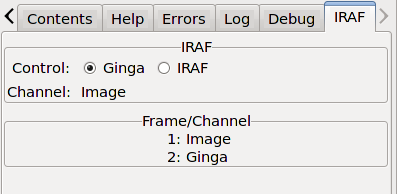
\includegraphics[width=4in]{IRAF-plugin.png}
    \end{tabular}
  \end{center}
  \caption[example] 
          { \label{fig:IRAF-plugin} 
            The IRAF plugin GUI.} 
\end{figure} 
The IRAF plugin allows Ginga to interoperate with IRAF in a manner
similar to IRAF and ds9.  The following IRAF commands are supported:
{\tt imexamine}, {\tt rimcursor}, {\tt display} and {\tt tvmark}.

To use the IRAF plugin, first make sure the environment variable IMTDEV
is set appropriately, e.g.
\begin{verbatim}
$ export IMTDEV=inet:45005         (or)
$ export IMTDEV=unix:/tmp/.imtg45
\end{verbatim}
If the environment variable is not set, Ginga will default to that used
by IRAF. 
    
Then start Ginga and IRAF.  For Ginga, the IRAF module is not loaded by
default.  To load it, specify the command line option:
\begin{verbatim}
--modules=IRAF
\end{verbatim}
In Ginga a GUI for the IRAF plugin, as shown in
Fig. \ref{fig:IRAF-plugin} will appear in the tabs on the right.

It can be more convenient to load images via Ginga than IRAF.  From
Ginga you can load images via drag and drop or via the FBrowser 
plugin and then use {\tt imexamine} from IRAF to do analysis tasks on
them.  You can also use the {\tt display} command from IRAF to show
images already loaded in IRAF in Ginga, and then use {\tt imexamine} to
select areas graphically for analysis.

When using {\tt imexamine} or {\tt rimcursor}, the plugin disables
normal UI processing on the channel image so that keystrokes,
etc. normally caught by Ginga are passed through to IRAF.  You can
toggle back and forth between local Ginga control (e.g. keystrokes to
zoom and pan the image, or apply cut levels, etc.) and IRAF control
using the radio buttons at the top of the tab.   

IRAF deals with images in enumerated ``frames'', whereas Ginga uses
named channels.  The bottom of the IRAF plugin GUI will show the mapping
from Ginga channels to IRAF frames, as seen in Fig. \ref{fig:IRAF-plugin}.

\chapter{Customizing Ginga}
\label{ch:customizing}
This chapter explains how you can customize Ginga in various ways.

\section{Rebinding Controls}
\label{sec:bindings}

\subsection{Example: ds9 bindings}
This example shows some code you can use to give ds9-like mouse bindings
to for colormap stretch (right mouse button) and setting pan position
(scroll button). This code can be added to the startup customization
script in \$HOME/.ginga/ginga\_config.py .

The standard Bindings class is subclassed, and we override the method
for the setup of the standard button events.  Two new methods are
provided for doing colormap tweaking and setting the pan position, both
without the usual onscreen message.  Care is taken to make sure that the
standard events used for plugins are not disrupted.

\begin{lstlisting}
from ginga.Bindings import FitsImageBindings
# uncomment the right one for your platform
#from ginga.gtkw.FitsImageGtk import FitsImageZoom
from ginga.qtw.FitsImageQt import FitsImageZoom

# subclass the standard bindings and rewire some things
# changes are NOTED

class MyGingaBindings(FitsImageBindings):

    def setup_default_btn_events(self, fitsimage, bindmap):

        # Generate standard symbolic mouse events for unmodified buttons:
        # xxxxx-{down, move, up}
        # e.g. 'left' button down generates 'cursor-down', moving the mouse
        # with no button pressed generates 'none-move', etc.
        for btnname, evtname in (('nobtn', 'none'), ('left', 'cursor'),
                                 ('middle', 'wheel'), ('right', 'draw')):
            bindmap.map_event(None, btnname, evtname)

        # standard bindings
        bindmap.map_event('shift', 'left', 'panset')
        bindmap.map_event('ctrl', 'left', 'pan')
        # NOTE: disable standard free panning, because we want middle click
        # to set pan position
        #bindmap.map_event(None, 'middle', 'freepan')
        bindmap.map_event(None, 'middle', 'panset')
        bindmap.map_event('ctrl', 'right', 'cmapwarp')
        bindmap.map_event('ctrl', 'middle', 'cmaprest')
        # name 'scroll' is hardwired for the scrolling action
        bindmap.map_event(None, 'scroll', 'zoom')
        bindmap.map_event('shift', 'scroll', 'zoom-fine')
        bindmap.map_event('ctrl', 'scroll', 'zoom-coarse')

        # Mouse operations that are invoked by a preceeding key
        for name in ('rotate', 'cmapwarp', 'cutlo', 'cuthi', 'cutall',
                        'draw', 'pan', 'freepan'):
            bindmap.map_event(name, 'left', name)

        # Now register our actions for these symbolic events
        # NOTE: disable standard cmapwarp, we want to call our own callback
        for name in ('cursor', 'wheel', 'draw', 'rotate', #'cmapwarp',
                     'pan', 'freepan', 'cutlo', 'cuthi', 'cutall'):
            method = getattr(self, 'ms_'+name)
            for action in ('down', 'move', 'up'):
                fitsimage.set_callback('%s-%s' % (name, action), method)
        # NOTE:
        # 1. bind draw to color map warp when it isn't captured by a plugin
        # 2. color warping is bound to my callback (below) to disable onscreen
        #      message
        for action in ('down', 'move', 'up'):
            fitsimage.set_callback('draw-%s' % (action), self.my_cmapwarp)
            # bind normal cmapwarp to my version (sans message)
            fitsimage.set_callback('cmapwarp-%s' % (action), self.my_cmapwarp)

        # NOTE: I don't want to see the onscreen pan position set message
        fitsimage.set_callback('panset-down', self.my_panset)
        fitsimage.set_callback('cmaprest-down', self.ms_cmaprest)

        fitsimage.set_callback('zoom-scroll', self.ms_zoom)
        fitsimage.set_callback('zoom-coarse-scroll',
                               self.ms_zoom_coarse)
        fitsimage.set_callback('zoom-fine-scroll', self.ms_zoom_fine)

    def my_panset(self, fitsimage, action, data_x, data_y):
        # set pan position, but suppress onscreen message
        return self.ms_panset(fitsimage, action, data_x, data_y,
                              msg=False)

    def my_cmapwarp(self, fitsimage, action, data_x, data_y):
        # warp color map, but suppress onscreen message
        return self.ms_cmapwarp(fitsimage, action, data_x, data_y,
                                msg=False)

def pre_gui_config(ginga):
    # this method is called before the GUI is brought up
    # custom configuration can be done here
    FitsImageZoom.set_bindingsClass(MyGingaBindings)
\end{lstlisting}

\section{Workspace configuration}
\label{sec:workspaceconfig}
Ginga has a flexible table-driven layout scheme for dynamically creating
workspaces and mapping the plugins to workspaces.  By changing a couple
of tables you can change the way Ginga looks and presents its content. 
If you examine the top-level startup script {\tt ginga.py} you will find
the tables: {\tt default\_layout}, {\tt global\_plugins} and
{\tt local\_plugins}.
global\_plugins and local\_plugins define the mapping of plugins to
workspaces and the titles on the tabs in the workspaces (if the
workspace has tabs--some don't).  
Here is an example of these two tables:
\begin{lstlisting}
global_plugins = [
    Bunch(module='Pan', tab='Pan', ws='uleft', raisekey='i'),
    Bunch(module='Info', tab='Info', ws='lleft', raisekey='i'),
    Bunch(module='Header', tab='Header', ws='left', raisekey='h'),
    Bunch(module='Zoom', tab='Zoom', ws='left', raisekey='z'),
    Bunch(module='Thumbs', tab='Thumbs', ws='right', raisekey='t'),
    Bunch(module='Contents', tab='Contents', ws='right', raisekey='c'),
    Bunch(module='WBrowser', tab='Help', ws='right', raisekey='?'),
    Bunch(module='Errors', tab='Errors', ws='right'),
    Bunch(module='Log', tab='Log', ws='right'),
    Bunch(module='Debug', tab='Debug', ws='right'),
    ]

local_plugins = [
    Bunch(module='Pick', ws='dialogs', shortkey='f1'),
    Bunch(module='Ruler', ws='dialogs', shortkey='f2'),
    Bunch(module='MultiDim', ws='dialogs', shortkey='f4'), 
    Bunch(module='Cuts', ws='dialogs', shortkey='f5'),
    Bunch(module='Histogram', ws='dialogs', shortkey='f6'),
    Bunch(module='PixTable', ws='dialogs', shortkey='f7'),
    Bunch(module='Preferences', ws='dialogs', shortkey='f9'),
    Bunch(module='Catalogs', ws='dialogs', shortkey='f10'),
    Bunch(module='Drawing', ws='dialogs', shortkey='f11'),
    Bunch(module='FBrowser', ws='dialogs', shortkey='f12'), 
    ]
\end{lstlisting}
The format of this table is simply a series of tuples''bunches''.
In the case of global\_plugins, each bunch specifies a module 
a title for the tab, the workspace that it should occupy, and an
optional key to raise that tab when pressed.
We can see that the ``Pan'' plugin will occupy the ``uleft'' workspace
and have a tab name of ``Pan'' (if that workspace has tabs).

Next we look at the default\_layout table:
\begin{lstlisting}
default_layout = ['hpanel', {},
                  ['ws', dict(name='left', width=320),
                   # (tabname, layout), ...
                   [("Info", ['vpanel', {},
                              ['ws', dict(name='uleft', height=300,
                                          show_tabs=False)],
                              ['ws', dict(name='lleft', height=430,
                                          show_tabs=False)],
                              ]
                     )]
                     ],
                  ['vbox', dict(name='main', width=700)],
                  ['ws', dict(name='right', width=400),
                   # (tabname, layout), ...
                   [("Dialogs", ['ws', dict(name='dialogs')
                                 ]
                     )]
                    ],
                  ]
\end{lstlisting}
This table defines how many workspaces we will have, their
characteristics, how they are organized, and their names.
The table consists again of a series of sublists or tuples, but in this
case they can be nested.
The first item in a sublist indicates the type of the container to be
constructed.  The following types are available:
\begin{itemize}
\item hpanel -- a horizontal panel of containers, with handles to size them
\item vpanel -- a vertical panel of containers, with handles to size
  them
\item hbox -- a horizontal panel of containers of fixed size
\item vbox -- a vertical panel of containers of fixed size
\item ws -- a workspace that allows a plugin gui or other items, usually
  implemented by a notebook-type widget
\item widget -- a preconstructed widget passed in
\end{itemize}
In every case the second item in the sublist is a dictionary that
provides some optional parameters that modify the characteristics of the
container.
If there is no need to override the default parameters the dictionary
can simply be empty.
The optional third and following items are specifications for nested
content.

All types of containers honor the following parameters:
\begin{itemize}
\item width -- can specify a desired width in pixels for the container.
\item height -- can specify a desired height in pixels for the container.
\item name -- specifies a mapping of a name to the created container
  widget.  The name is important especially for workspaces, as they may
  be referred to in the default\_tabs table.
\end{itemize}

In the above example, we define a top-level horizontal panel of three
containers: a workspace named ``left'' with a width of 320 pixels, a
vertical fixed container named ``main'' with a width of 700 pixels and a
workspace called ``right'' with a width of 400 pixels.  The ``left''
workspace is pre-populated with an ``Info'' tab containing a vertical
panel of two workspaces: ``uleft'' and ``lleft'' with heights of 300 and
430 pixels, respectively, and neither one should show tabs.  The ``right''
workspace is pre-populated with a ``Dialogs'' tab containing an empty
workspace.  Looking back at the  default\_tabs table you can now more 
clearly see how the mapping of plugins to workspaces is handled through
the names.

Ginga uses some container names in special ways.
For example, the ``main'' container is populated by Ginga with the tabs
for each channel, and the ``dialogs'' workspace is where all of the
local plugins are instantiated (when activated).
These two names should at least be defined somewhere in default\_layout.

\section{Writing a global plugin}
\label{sec:globalplugins}
Global plugins are basically treated like mini programs that get loaded
into Ginga and are started when the program starts\footnote{If the
  plugin is not listed in the default\_tabs table described in section
  \ref{sec:workspaceconfig} it won't be started at program startup.}.
A global plugin does not need to have a user interface associated with
it.  

Global plugins are best suited for adding features to Ginga that
should operate ``across channels''; i.e. some visible interface that
continuously updates itself in response to events happening in the
viewer.

The API for a global plugin is pretty simple.  This template shows the
relevant class definition:
\begin{lstlisting}
class Foo(GingaPlugin.GlobalPlugin):
    """
    NOTE: *** All these methods are running in the GUI thread, unless
    otherwise noted. Do not block!! ***  
    """

    def __init__(self, fv):
        super(Foo, self).__init__(fv)

        # Hereafter, in this object we can refer to:
        # self.fv -- the main Ginga control object
        # self.logger -- a logger

    def initialize(self, container):
        """This method will be called with a container widget if the global
        plugin was requested to be loaded into a workspace.  The plugin should
        construct its GUI and pack it into the container.  If there is
        no GUI for the global plugin this method can be omitted.
        """
        pass

    def start(self):
        """This method is called just after build_gui() when the plugin is
        activated (for global plugins this is usually at program start up).
        For global plugins this method can often be omitted.
        """
        pass

    def stop(self):
        """This method is called when the plugin is deactivated.
        For global plugins this method can usually be omitted.
        """
        pass

    def pause(self):
        """If present, this method can be called to defocus the plugin
        without stopping it.  
        For global plugins this method can usually be omitted.
        """
        pass

    def resume(self):
        """If present, this method can be called to focus the plugin
        subsequent to a previous pause() call.  
        For global plugins this method can usually be omitted.
        """
        pass
\end{lstlisting}
There is the object constructor, an {\tt build\_gui} method and 
{\tt start} and {\tt stop} methods.  
Global plugins register with the main ginga object for events they
are interested in, like when a channel is added, or a new image arrives
in a channel, and define their own callbacks to deal with them.  This is
typically done in the constructor, although it can also be done in the
{\tt build\_gui} method.  The start, stop, pause and resume methods are
currently reserved for future use and can be omitted. 

The best way to learn how a global plugin interacts with the main Ginga
control object (represented by the {\tt fv} parameter in the
constructor) is to examine some of the global plugins that ship with
Ginga.  Start with a simple one, like Header, and work up to more
complicated examples like Info.

\section{Writing a local plugin}
\label{sec:localplugins}
Local plugins are also more or less independent modules that are loaded
into Ginga at program startup, but there is a unique instance of a local
plugin for each channel.  Local plugins are also more tightly controlled
by Ginga: they create their user interface (if any) when the plugin
is activated, and it disappears when the plugin is deactivated.
Furthermore, while the plugin is activated it may lose or regain the
focus, which generally serves to multiplex the keyboard and mouse
operations amongst the different active local plugins.  
Local plugins are activated, deactivated and focus-controlled via the 
plugin manager bar that appears at the bottom of the main FITS window.

Here is a template for a local plugin.  As you can see, the API is a
little more complicated than for a global plugin, but not by much.
\begin{lstlisting}
class Goo(GingaPlugin.LocalPlugin):
    """
    NOTE: *** All these methods are running in the GUI thread, unless
    otherwise noted. Do not block!! ***  
    """

    def __init__(self, fv, fitsimage):
        super(Goo, self).__init__(fv, fitsimage)

        # Hereafter, in this object we can refer to:
        # self.fv -- the main Ginga control object
        # self.fitsimage -- the channel viewer object we are associated with
        # self.logger -- a logger

    # def build_gui(self, container):
    #     """If a plugin defines this method, it will be called with a
    #     container object in which to build its GUI. It should finish
    #     by packing into this container.  This will be called every
    #     time the local plugin is activated.
    #     """
    #     pass

    def start(self):
        """This method is called just after build_gui() when the plugin is
        activated.
        """
        pass
        
    def stop(self):
        """This method is called when the plugin is deactivated.
        """
        pass

    def pause(self):
        """This method is called when the plugin is defocused.  The plugin
        should disable any user input that it responds to.
        """
        pass

    def resume(self):
        """This method is called when the plugin is focused.  The plugin
        should enable any user input that it responds to.
        """
        pass

    def redo(self):
        """This method is called when a new image arrives in the channel
        associated with the plugin.  It can optionally redo whatever operation
        it is doing.
        """
        pass
\end{lstlisting}

The best way to learn how a local plugin interacts with the main Ginga
control object (the {\tt fv} parameter in the constructor) and the local
channel image ({\tt fitsimage}) is to examine some of the local plugins
that ship with Ginga.  Start with a simple one, like Ruler or Drawing,
and work up to more complicated examples like Pick or Catalogs.

\chapter{Ginga Programming Internals}
\label{ch:internals}
This chapter explains the secret inner workings of Ginga and its widgets
so that you can subclass them and use them in your own applications.

\emph{TBD}

\section{Architecture}

\emph{TBD}

%%%%%%%%%%%%%%%%%%%%%%%%%%%%%%%%%%%%%%%%%%%%%%%%%%%%
\appendix    %>>>> this command starts appendixes
%%%%%%%%%%%%%%%%%%%%%%%%%%%%%%%%%%%%%%%%%%%%%%%%%%%%

\chapter{Keyboard and Mouse Quick Reference}
\label{app:mousekbdref}

\section{Main image window}
These keyboard and mouse operations are available when the main image
window has the focus.

\subsection{Panning and Zooming commands}
\begin{tabularx}{\textwidth}{lX}
Scroll wheel turned & Zoom in or out \\
Digit ({\tt 1234567890}) & Zoom image to zoom steps 1, 2, ..., 9, 10 \\
Shift + Digit & Zoom image to zoom steps -1, -2, ..., -9, -10 \\
Backquote (\`{}) & Zoom image to fit window \\
Minus, Underscore ({\tt -\textunderscore{}}) & Zoom out \\
Equals, Plus ({\tt =+}) & Zoom in \\
Middle (scroll) button drag & Pan image freely (when zoomed in) \\
{\tt p} & Set pan position for zooming \\
Shift + Left click & Set pan position for zooming \\
{\tt c} & Set pan position to the center of the image \\
{\tt q} & Pan image freely (when zoomed in); move mouse (no button press); left click to terminate) \\
Ctrl + Left drag & Proportional pan (press and drag left mouse button) \\
apostrophe ({\tt '}) & Set autozoom for new images to {\em override} \\
doublequote ({\tt ''}) & Set autozoom for new images to {\em on} \\
Ctrl + Scroll wheel turned & Adjust zoom by intermediate coarse steps \\
Shift + Scroll wheel turned & Adjust zoom by intermediate fine steps \\
\end{tabularx}

\subsection{Cut levels and colormap commands}
\begin{tabularx}{\textwidth}{lX}
{\tt a} & Auto cut levels \\
left angle ({\tt \textgreater{}}) & Interactive cut low (with left mouse button) \\ 
right angle ({\tt \textless{}}) & Interactive cut high (with left mouse button) \\ 
period ({\tt .}) & Interactive cut \emph{both} low and high (with left mouse button) \\ 
slash ({\tt /}) & Interactive warp colormap (with left mouse button) \\
semicolon ({\tt ;}) & Set autocuts for new images to {\em override} \\
colon ({\tt :}) & Set autocuts for new images to {\em on} \\
question ({\tt ?}) & Restore the color map to its original state \\
\end{tabularx}

\subsection{Transform commands}
\begin{tabularx}{\textwidth}{lX}
Left bracket ({\tt [}) & Flip image in X \\
Left brace ({\tt \textbraceleft{}}) & Restore image in X \\
Right bracket ({\tt ]}) & Flip image in Y \\
Right brace ({\tt \textbraceright{}}) & Restore image in Y \\
Backslash ({\tt \textbackslash{}}) & Swap X and Y axes \\
Vertical bar ({\tt \textbar{}}) & Restore X and Y axes \\
{\tt r} & Interactive rotate (with left mouse button) \\
{\tt R} & Restore rotation to 0 degrees \\
\end{tabularx}

\subsection{Tab Navigation}
\begin{tabularx}{\textwidth}{lX}
{\tt I} & Raise Info tab \\
{\tt H} & Raise Header tab \\
{\tt Z} & Raise Zoom tab \\
{\tt D} & Raise Dialogs tab \\
{\tt T} & Raise Thumbs tab \\
{\tt C} & Raise Contents tab \\
\end{tabularx}

%% \subsection{Plugins}
%% \begin{tabularx}{\textwidth}{llX}
%% Escape & Stop current plugin operation & \\
%% {\tt F1} & Start Pick & Stellar evaluation \\
%% {\tt F2} & Start Ruler & Measure distances \\
%% {\tt F3} & (Reserved for future use) & \\
%% {\tt F4} & Start MultiDim & Browse HDUs and image slices \\
%% {\tt F5} & Start Cuts & Graph pixel values along a line \\
%% {\tt F6} & Start Histogram & Graph pixel values in a region \\
%% {\tt F7} & Start PixTable & Show maxtrix of pixel values around cursor \\
%% {\tt F8} & (Reserved for future use) & \\
%% {\tt F9} & Start Preferences & Set preferences for a channel \\
%% {\tt F10} & Start Catalog & Access image and star catalogs \\
%% {\tt F11} & Start Drawing & Draw graphics on an image \\
%% {\tt F12} & Start FBrowser & Browse and load files \\
%% \end{tabularx}

If there are one or more plugins active, additional mouse or keyboard
bindings may be present.  In general, the left mouse button is used to
select, pick or move, and the right mouse button is used to draw a
shape for the operation.  
On the Mac, control + mouse button can also be used to draw or right click.

\chapter{Miscellanea}
\section{Etymology}
``Ginga'' is the romanized spelling of the Japanese word ``銀河''
(hiragana: ぎんが), meaning ``galaxy'' (in general) and, more familiarly,
the Milky Way.  This viewer was written by software engineers at Subaru
Telescope, National Astronomical Observatory of Japan--thus the
connection. 

\section{Pronunciation}
Ginga the viewer may be pronounced ``ging-ga'' (proper japanese) or
``jing-ga'' (perhaps easier for western tongues).  The latter
pronunciation has meaning in the Brazilian dance/martial art
\emph{capoeira}: a fundamental rocking or back and forth swinging
motion.
Note: pronunciation as ``gin-ja'' is particularly bad form!

\end{document} 
